\chapter{Experimental Design and Results}
\label{chap:results}

\begin{quote}
\textbf{Scope of this evaluation.} The results below were produced by the
accompanying \texttt{evaluate.py} on the two datasets described in
Section~\ref{sec:datasets}. Both are non-standard: a procedurally generated
\emph{structured} image set and the offline scikit-learn \emph{digits}
dataset. They are used because the evaluation environment had no network
access to standard vision benchmarks (e.g.\ CIFAR-10). Consequently, the
numbers below are genuine measurements of the training dynamics and
resource cost of the architecture, but they are \emph{not} benchmark
accuracy results, and no classification accuracy is claimed. Evaluation on
a standard benchmark remains future work (Chapter~\ref{chap:conclusion}).
\end{quote}

\section{Research Questions}
\begin{description}
    \item[RQ1 (Collapse):] Does the variance/covariance regularization
    prevent representational collapse relative to an unregularized
    ($\alpha = \beta = 0$) JEPA?
    \item[RQ2 (Efficiency):] What are the inference latency and memory
    footprint of EdgeVerify?
    \item[RQ3 (Convergence):] Does the local objective converge stably?
\end{description}

\section{Experimental Setup}
All experiments were run on a single cloud CPU (two threads, no GPU) using
PyTorch~2.14. The architecture and optimizer follow Chapter~\ref{chap:method}
exactly (Table~\ref{tab:hparams}). Each configuration was trained with a
single random seed; multi-seed repetition is noted as a limitation in
Section~\ref{sec:threats}. Table~\ref{tab:setup} lists the run
configuration.

\begin{table}[htbp]
    \centering
    \caption{Evaluation configuration.}
    \label{tab:setup}
    \begin{tabular}{ll}
        \toprule
        \textbf{Item} & \textbf{Value} \\
        \midrule
        Framework / device & PyTorch 2.14, CPU (2 threads) \\
        Optimizer & AdamW ($10^{-3}$, weight decay $10^{-4}$) \\
        Batch size & $64$ \\
        Epochs (structured / digits) & $40$ / $25$ \\
        Samples (structured / digits) & $768$ / $1797$ \\
        Seeds & $1$ (single seed) \\
        \bottomrule
    \end{tabular}
\end{table}

\section{Datasets}
\label{sec:datasets}
\paragraph{Structured.} Each $64\times64$ RGB image is generated with a
random background gradient and one to three random rectangles and circles,
yielding genuine local spatial structure (in contrast to the i.i.d.\ noise
used in the initial smoke test). The context view is produced by zeroing a
random rectangular region occupying $35$--$60\%$ of each side, and the
spatial action is the normalized bounding box of that region.

\paragraph{Digits.} The scikit-learn handwritten-digits dataset ($1797$
real $8\times8$ images) is upsampled to $64\times64$ and replicated to
three channels. It provides a small but \emph{real} data source available
without network access, used as a sanity check. The same random masking is
applied.

\section{Evaluation Metrics}
Two collapse indicators are computed over the context embedding
$s_t \in \mathbb{R}^{d}$ ($d = 256$) on up to $512$ samples:
\begin{itemize}
    \item \textbf{Mean embedding std} $\bar\sigma = \frac{1}{d}\sum_j
    \sqrt{\operatorname{Var}(s_{t,j})}$. Variance collapse drives
    $\bar\sigma \rightarrow 0$.
    \item \textbf{Effective rank} (participation ratio)
    $\big(\sum_i \lambda_i\big)^2 / \sum_i \lambda_i^2$, where $\lambda_i$
    are the eigenvalues of the embedding covariance. Dimensional collapse
    (correlated dimensions) drives this toward $1$.
\end{itemize}
Efficiency is reported as parameter count, parameter memory, and
single-sample inference latency (mean $\pm$ std over $50$ runs after
warm-up).

\section{Results}

\subsection{Convergence and Collapse (RQ1, RQ3)}
Table~\ref{tab:convergence} reports the final loss and collapse indicators;
Figure~\ref{fig:losscurves} shows the training curves and
Figure~\ref{fig:collapse} the collapse indicators.

\begin{table}[htbp]
    \centering
    \caption{Convergence and collapse indicators. $\mathcal{L}_{\text{total}}$
    and $\mathcal{L}_{\text{distill}}$ are the final-epoch values;
    $\bar\sigma$ and effective rank are measured on the trained context
    encoder. A lower $\mathcal{L}_{\text{distill}}$ is not necessarily
    better---see the discussion.}
    \label{tab:convergence}
    \begin{tabular}{llcccc}
        \toprule
        \textbf{Data} & \textbf{Model} &
        $\mathcal{L}_{\text{total}}$ & $\mathcal{L}_{\text{distill}}$ &
        $\bar\sigma$ & \textbf{Eff.\ rank} \\
        \midrule
        \multirow{2}{*}{Structured}
          & Unregularized ($\alpha{=}\beta{=}0$) & $0.0021$ & $0.0021$ & $0.245$ & $6.46$ \\
          & EdgeVerify (full)                    & $0.190$  & $0.120$  & $\mathbf{1.549}$ & $1.64$ \\
        \midrule
        \multirow{2}{*}{Digits}
          & Unregularized ($\alpha{=}\beta{=}0$) & $0.0006$ & $0.0006$ & $0.080$ & $3.57$ \\
          & EdgeVerify (full)                    & $0.257$  & $0.207$  & $\mathbf{1.772}$ & $1.03$ \\
        \bottomrule
    \end{tabular}
\end{table}

\begin{figure}[htbp]
    \centering
    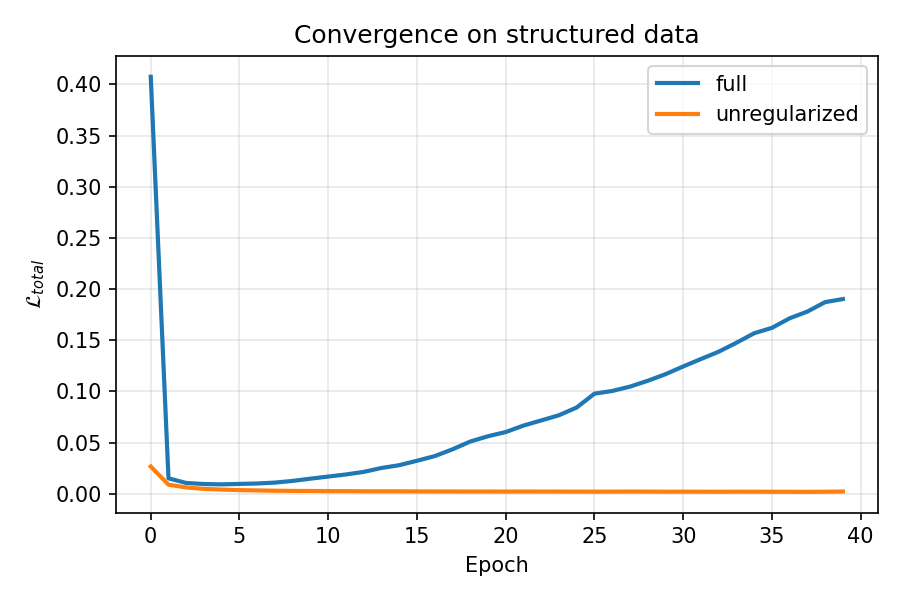
\includegraphics[width=0.49\textwidth]{images/loss_curves_structured.png}
    \hfill
    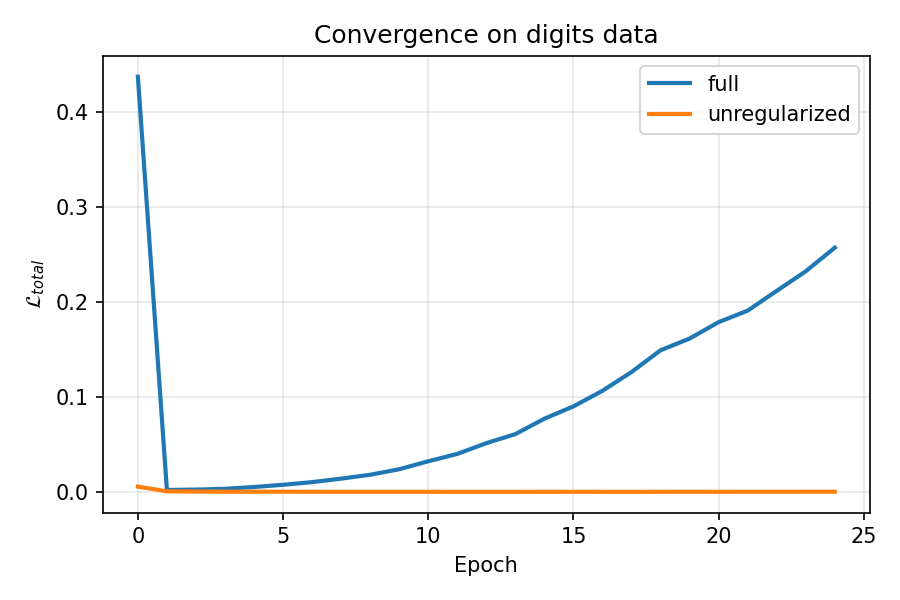
\includegraphics[width=0.49\textwidth]{images/loss_curves_digits.png}
    \caption{Total-loss convergence for the full objective and the
    unregularized baseline. The unregularized objective (distillation only)
    is trivially driven toward zero, whereas the full objective is
    non-monotonic: after the distillation term is minimized, the aggregate
    rises as the (weakly weighted) covariance term grows.}
    \label{fig:losscurves}
\end{figure}

\begin{figure}[htbp]
    \centering
    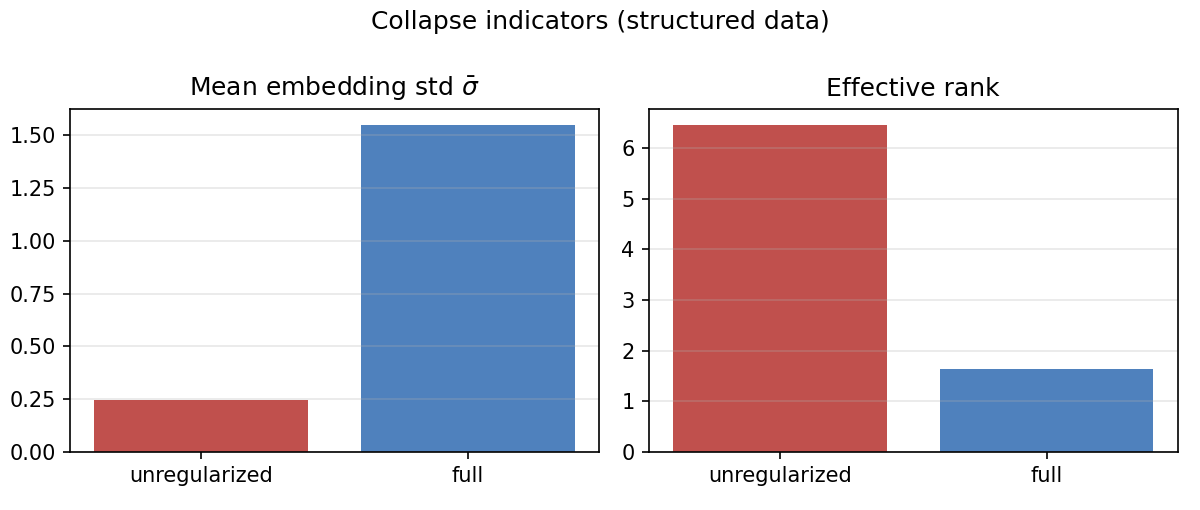
\includegraphics[width=0.49\textwidth]{images/collapse_bars_structured.png}
    \hfill
    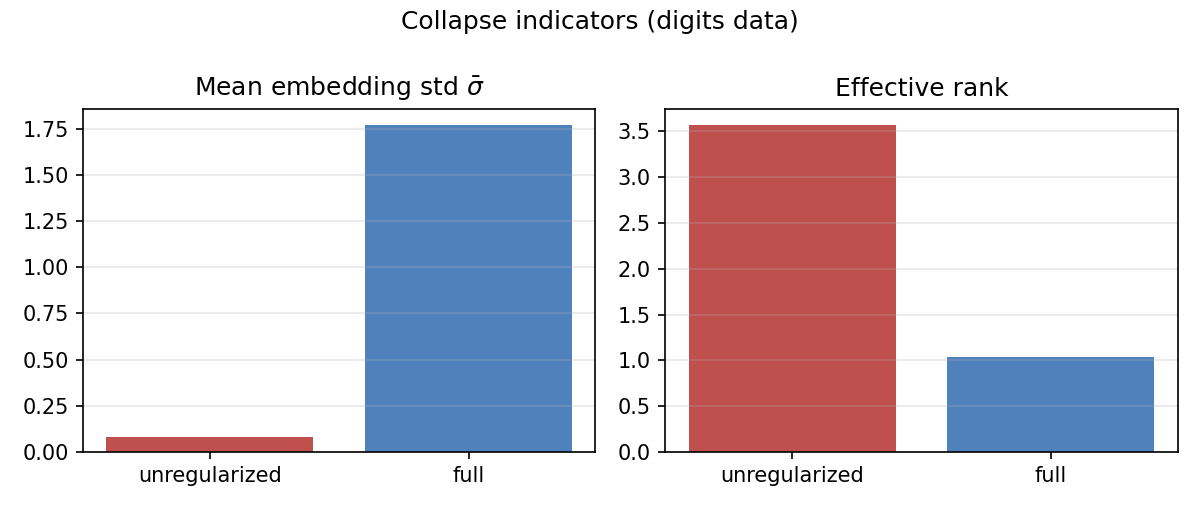
\includegraphics[width=0.49\textwidth]{images/collapse_bars_digits.png}
    \caption{Collapse indicators. The variance term sustains a high mean
    embedding standard deviation $\bar\sigma$, but the effective rank of the
    full model is lower than that of the unregularized baseline.}
    \label{fig:collapse}
\end{figure}

The results are mixed and warrant careful reading. The variance regularizer
is effective at its stated objective: the full model maintains
$\bar\sigma \approx 1.55$--$1.77$, at or above the hinge threshold
$\gamma = 1.0$ (its final variance-loss term reaches $\approx 0$), whereas
the unregularized baseline collapses toward low per-dimension variance
($\bar\sigma = 0.245$ and $0.080$). This directly confirms that the
variance term prevents the low-variance mode of collapse.

However, the \emph{effective rank} tells the opposite story: the full model
attains a very low effective rank ($1.64$ and $1.03$ out of $256$), and it
is in fact \emph{lower} than the unregularized baseline ($6.46$ and $3.57$).
High per-dimension variance therefore coexists with strongly correlated
dimensions---a rank-deficient representation. At the code's covariance
weight $\beta = 0.01$, the decorrelation term is too weak to counteract this,
which is consistent with the growing covariance component visible in
Figure~\ref{fig:losscurves}. \textbf{The regularization as configured
prevents variance collapse but does not, on this evidence, prevent
dimensional (rank) collapse.}

\subsection{Efficiency (RQ2)}
Table~\ref{tab:efficiency} reports the model's cost. The architecture is
compact---$745{,}536$ parameters, $2.84$~MB of parameter memory---and
achieves single-sample inference in roughly $2$~ms on CPU.

\begin{table}[htbp]
    \centering
    \caption{Inference latency and memory. Peak RSS reflects the full
    PyTorch process (runtime libraries dominate) and is reported only as a
    coarse proxy; the model's own parameter memory is the meaningful
    edge-relevant figure.}
    \label{tab:efficiency}
    \begin{tabular}{lcccc}
        \toprule
        \textbf{Data} & \textbf{Params} & \textbf{Param mem.\ (MB)} &
        \textbf{Latency (ms)} & \textbf{Peak RSS (MB)} \\
        \midrule
        Structured & $745{,}536$ & $2.84$ & $2.04 \pm 0.11$ & $852$ \\
        Digits     & $745{,}536$ & $2.84$ & $2.48 \pm 0.53$ & $1099$ \\
        \bottomrule
    \end{tabular}
\end{table}

\section{Discussion}
On RQ1, the evidence is partial: the variance constraint demonstrably
mitigates variance collapse, but at $\beta = 0.01$ the covariance constraint
does not yield a high-rank representation, and the unregularized baseline is
paradoxically higher-rank. A plausible explanation is that the variance and
covariance penalties act on different tensors (the context embedding $s_t$
and the prediction $s_{\text{pred}}$, respectively; Chapter~\ref{chap:method})
and that the covariance weight is an order of magnitude too small relative to
the variance weight. This motivates a dedicated $\beta$ ablation, listed as
future work. On RQ2, the architecture is genuinely lightweight ($2.84$~MB of
parameters, millisecond CPU inference), supporting its suitability for
edge deployment in terms of size. On RQ3, the distillation term converges
rapidly in all cases; the full objective's total loss is non-monotonic
because the covariance term grows once distillation is satisfied.

Notably, the unregularized baseline attains a far lower total loss
($\sim 10^{-3}$) precisely because, with $\alpha = \beta = 0$, the objective
reduces to distillation MSE, which is trivially minimized while the
representation quietly loses variance. This is a concrete illustration of
why loss magnitude alone is an inadequate proxy for representation quality,
and why the collapse indicators are necessary.

\section{Threats to Validity}
\label{sec:threats}
Several factors limit the strength of these conclusions: (i) the datasets are
non-standard (synthetic structured images and low-resolution real digits),
so results may not transfer to natural-image benchmarks; (ii) each
configuration was run with a single seed, so run-to-run variance is not
quantified; (iii) all measurements are CPU-only, so latency and memory would
differ on target embedded hardware; and (iv) the encoder is small relative to
the transformer backbones typical of the JEPA literature. Addressing these is
the subject of Chapter~\ref{chap:conclusion}.
